\documentclass[12pt, a4paper]{article}
\usepackage[utf8]{inputenc}
\usepackage{indentfirst} %indentace prvního odstavce
\usepackage{url}
\usepackage{amsmath}
\usepackage{graphicx}
\graphicspath{ {doc-img/} }

\title{OOP Zápočtový program - Diskrétní simulace metra}
\author{Jan Oupický}
\date{2018}

\begin{document}
\maketitle

\section{Zadání}

Program má za úkol provést diskrétní simulaci metra. Cílem této simulace bude zjištění doby cesty ze stanice A do stanice B za různých podmínek jako kapacita souprav, počet lidí, počet souprav apod. 

\section{Uživatelský manuál}

Spolu s programem je distibuován soubor \url{stanice.txt}, ve kterém je seznam stanic metra. Základně je v něm seznam stanic pražského metra v požadovaném formátu.

Uživatel si ale může tento soubor upravit podle libosti, akorát musí dodržet následující syntaxi:

\begin{itemize}
    \item Prázdné řádky jsou ignorovány.
    \item Řádek, který začíná "\#" je komentář. Tento řádek je také ignorován
    \item Na každém řádku se může nacházet pouze jedna stanice metra.
    \item Řádek se stanicí musí mít následujicí formát:
    \[ % hack pro posunuti doleva
    \displayindent0pt
    \displaywidth\textwidth
    \mathtt{[pismeno], [nazev], [km], [je\;konecna], [je\;prestupni], [prestupni\;pismeno]}\text{, kde}
    \]
    \texttt{[pismeno]} = Písmeno linky, na které se daná stanice nachází\\
    \texttt{[nazev]} = Název stanice\\
    \texttt{[km]} = Na kolikátém kilometru od počáteční stanice se stanice nachází. Počáteční stanice má 0. kilometr. Číslo může být i s desetinnou tečkou.\\
    \texttt{[je konecna]} = Zda je stanice konečná. 0 = ne, 1 = ano. Tento údaj není povinný (defaultně je 0)\\
    \texttt{[je prestupni]} = Zda je stanice přestupní. 0 = ne, 1 = ano. Tento údaj není povinný (defaultně je 0)\\
    \texttt{[prestupni pismeno]} = Písmeno linky, na kterou lze z dané stanice přestoupit. Tento údaj není povinný, pokud je předchozí údaj 0.\\
    Řádky mohou tedy vypadat např. takto:
    \begin{verbatim}
    C, Háje, 0, 1
    B, Českomoravská, 6.4
    B, Florenc, 10.9, 0, 1, C
    \end{verbatim}
\end{itemize}

Poté již stačí program spustit a vybrat počáteční a konečnou stanici. Uživatel může dále měnit více specifická nastavení:
\begin{itemize}
    \item "Čas přichodu": Kdy dorazíme do počáteční stanice od prvního výjezdu souprav. První soupravy totiž vyjedou v čase 0 z konečných stanic. Zbylé soupravy vyjíždějí po 5 minutových intervalech.
    \item "Hustota lidí": Kolik lidí příjde každou minutu do metra (každý do náhodné stanice).
    \item "Linka": Výběr linky, pro kterou chceme měnit další nastavení.
    \item "Rychost soupravy": Rychlost souprav na dané lince v kilometrech za minutu.
    \item "Počet souprav": Počet souprav na dané lince. Počet souprav je sudý, jelikož soupravy vyrážejí po párech z konečných stanic.
    \item "Kapacita soupravy": Kolik lidí se vejde do jedné soupravy.
    \item "Doba čekání ve stanici": Jak dlouho souprava čeká ve stanici v minutách.
\end{itemize}

Hodnoty "Hustota lidí" a "Kapacita soupravy" by měly být upraveny oproti reálným hodnotám. Například v pražském metru ve špičce příjde do metra cca 1200 lidí za minutu. Každá souprava má kapacitu zhruba 1400. Základní nastavení je odvozeno od těchto údajů. Nechceme simulovat všech 1200 různých lidí za minutu ale stačí nám zhruba $\frac{1}{20}$, tedy "Hustota lidí" = 50 a "Kapacita soupravy" = 70.

Po nastavení stačí stisknout tlačítko "Simuluj" a počkat na výsledek, který se objeví pod tlačíkem. Uživatel po skončení jedné simulace může změnit nastavení a simulaci opakovat opětovným stiskem tlačítka.
\begin{figure}[h]
\centering
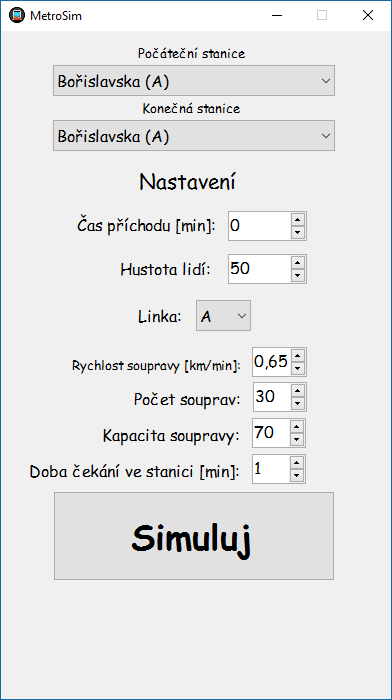
\includegraphics[scale=0.5]{obr1}
\caption{GUI programu}
\end{figure}
\section{Jak program funguje (algoritmus)}
Tak
\section{Implementace}

\end{document}